\chapter{Introduction}
\label{sec:intro}

% Die Einleitung schreibt man zuletzt, wenn die Arbeit im Großen und
% Ganzen schon fertig ist. (Wenn man mit der Einleitung beginnt - ein
% häufiger Fehler - braucht man viel länger und wirft sie später doch
% wieder weg). Sie hat als wesentliche Aufgabe, den Kontext für die
% unterschiedlichen Klassen von Lesern herzustellen. Man muß hier die
% Leser für sich gewinnen. Das Problem, mit dem sich die Arbeit befaßt,
% sollte am Ende wenigsten in Grundzügen klar sein und dem Leser
% interessant erscheinen. Das Kapitel schließt mit einer Übersicht über
% den Rest der Arbeit. Meist braucht man mindestens 4 Seiten dafür, mehr
% als 10 Seiten liest keiner.

The parallel execution of tasks was a problem in the past, and it remains so throughout the present day.
Imagine two checkout lanes running next to each other.
One serves customer by customer slowly but steadily, while the other empties out twice as fast.
The staff have different working speeds, the clients have varying numbers of items in their carts, and the cashier queues have differing lengths.
All those conditions lead to one usually choosing a suboptimal line for being processed as fast as possible.
A similar situation was experienced in the early \nth{20} century by telephone exchange centers.
Calls arrived at random, each one occupied a line for an arbitrary duration, and only a finite number of lines were available.
Additionally, each needed to be staffed by an operator.
The task the Danish mathematician Agner Krarup Erlang was faced with when working at the Copenhagen Telephone Company was how many circuits and operators the exchange needed for an expected volume of traffic while keeping the probability of a blocked call below an acceptable threshold.
As hold queues did not yet exist, callers were simply turned away when every line was occupied.
Hence, the goal was to minimize the number of blocked calls and, later, to reduce the waiting time in a hold queue as far as possible.
To solve those problems, Erlang introduced the field of queueing theory modeling such systems.\\

Time advanced, and so did technology, but the problems remained.
While modern telecommunication has since solved the problem for exchange centers as calls are now routed digitally, without manual operation, picking a checkout queue remains a task every customer still has to solve alone.

Further, this abstraction carries over almost directly into computing. A single processor core working through a stream of incoming tasks is structurally identical to a checkout lane with one cashier.
The jobs arrive, occupy the core for a finite duration, and are served in some order.
This uniprocessor case is well understood because decades of operating systems research have produced reliable scheduling strategies from round-robin to multilevel feedback queues.
They answer the question of who runs next when there is exactly one queue and one server.

The introduction of multiple processor cores changed comparatively little at first.
Several identical cores amount to several identical checkout lanes.
They are uniform in speed, each equally suited to any job.
Distributing work across them stays close to the classical queuing problem, where a job, like a customer, needs only be routed to whichever lane is shortest or fastest to clear.

\begin{figure}[h]
	\centering
	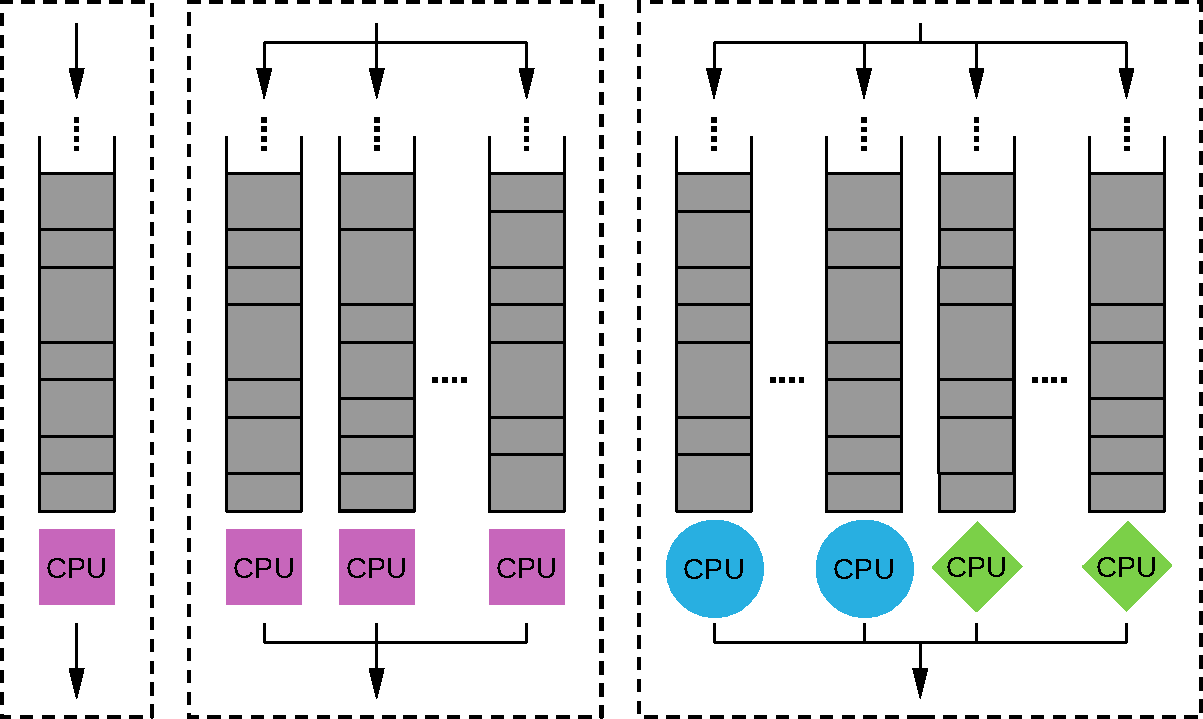
\includegraphics[width=0.75\textwidth]{images/queue_processing.pdf}
	\caption{Three queuing configurations: a single server (left), multiple servers of uniform speed (center), and multiple servers of asymmetric speed (right), illustrating the transition from uniprocessor to heterogeneous architecture scheduling.}
	\label{fig:queue-processing}
\end{figure}

This assumption of uniformity breaks down with modern processor chips. Contemporary hardware increasingly combines cores of different sizes and speeds on a single chip, so-called heterogeneous multiprocessing.
Doing so trades uniform performance for energy efficiency and workload-specific throughput.
Just as an operator once decided which caller was connected to which line, it is now the operating system's task to decide which job is assigned to which core.
Every incoming job must be routed not merely to any free queue, but to the queue best suited to both the job and the current state of the system.
This decision needs to be made anew for every single job rather than once for the system as a whole.
Unlike a shopper, the operating system cannot simply glance down the line and estimate how long a job will take.
It must decide under incomplete information, and unlike a customer changing lanes, moving a job from one queue to another is never free.\\

Queueing theory already distinguishes between two such decisions, even if the checkout analogy blurs them together.
It separates the question of who is served next within a line from the question of which line a new arrival should join.
The former defines the field of scheduling theory, and within an operating system, the component concerned with this decision is called a scheduler.
The latter is usually a subsystem of the scheduler, and its task is to balance load across the system; hence, the name load balancing.
As core responsibilities of every operating system, both must be designed to meet the demands of the workloads they serve.
This thesis is not about how work is ordered for a single server but about the strategy that distributes work among the available processing units.
Load balancing can pursue different goals, among them throughput, responsiveness, energy efficiency, and fairness.
Because these goals often conflict, a careful choice must be made before any implementation begins.
Designing such a balancing component becomes notably harder in microkernel-based operating systems, a challenge this thesis returns to once the relevant architectural background has been introduced.
Concretely, this thesis develops and evaluates a load-balancing component for the L4Re microkernel's userland that is aware of heterogeneous architecture, making the following contributions:

\begin{itemize}
	\item Design and implementation of a load balancing component for the L4Re userland
	\item Investigation of metrics suited to balancing load across heterogeneous cores
	\item Extension of L4Re microkernel interfaces where required by the design
	\item Selection of benchmarks, development of a benchmarking harness, and construction of dedicated test cases
	\item Evaluation of multiple load balancer configurations against Linux's EEVDF scheduler
\end{itemize}

\section{Outline}

This work is structured as follows.
Chapter~\ref{sec:state} introduces the terminology used throughout the thesis and surveys related work on load balancing in general-purpose, AMP, and microkernel-based operating systems. It then examines microkernel architecture in more depth, covering inter-process communication, scheduling, and heterogeneous hardware.
Chapter~\ref{sec:design} presents the design of the load balancing component developed in this thesis, including an architectural overview of its key components, their behavior, and how the design accounts for the constraints of the underlying microkernel architecture.
Chapter~\ref{sec:implementation} discusses challenges encountered during the implementation, extends the design with concepts from distributed systems, and describes tested optimizations.
Chapter~\ref{sec:evaluation} evaluates the resulting load balancer, comparing multiple configurations of the service against the Linux EEVDF scheduler on a set of selected benchmarks and purpose-built test cases.
Chapter~\ref{sec:futurework} outlines directions for extending, investigating, and optimizing the developed system, and Chapter~\ref{sec:conclusion} closes the thesis with a conclusion.

\cleardoublepage

%%% Local Variables:
%%% TeX-master: "diplom"
%%% End:
